
\documentclass[table]{beamer}

\mode<presentation> {
\usetheme{Madrid}

% changes the colors of your current slide theme.

%\usecolortheme{albatross}
%\usecolortheme{beaver}
%\usecolortheme{beetle}
%\usecolortheme{crane}
%\usecolortheme{dolphin}
%\usecolortheme{dove}
%\usecolortheme{fly}
%\usecolortheme{lily}
%\usecolortheme{orchid}
%\usecolortheme{rose}
%\usecolortheme{seagull}
%\usecolortheme{seahorse}
%\usecolortheme{whale}
%\usecolortheme{wolverine}

%\setbeamertemplate{footline} % To remove the footer line in all slides uncomment this line
%\setbeamertemplate{footline}[page number] % To replace the footer line in all slides with a simple slide count uncomment this line

%\setbeamertemplate{navigation symbols}{} % To remove the navigation symbols from the bottom of all slides uncomment this line
}

\usepackage{graphicx} % Allows including images
\usepackage{booktabs} % Allows the use of \toprule, \midrule and \bottomrule in tables

\usepackage{pifont}
\usepackage[english]{babel}
\usepackage{amssymb}
\usepackage{amsmath}
\usepackage[most]{tcolorbox}
%----------------------------------------------------------------------------------------
%	TITLE PAGE
%----------------------------------------------------------------------------------------

\title[Thesis Proposal]{Multi-Tier Priority Queues \& 2-Tier Ladder Queue for Managing Pending Events} % The short title appears at the bottom of every slide, the full title is only on the title page

\author{Julius D. Higiro} 
\institute[MU]
{
Miami University 
\medskip
}
\date{\today} 

\begin{document}

\begin{frame}
\titlepage 
\end{frame}

\begin{frame}
\frametitle{Overview} 
\tableofcontents 
\end{frame}
\section{Introduction}
\section{Research Motivation}
\section{Research Proposal}
\section{Related Work}
\section{Parallel Simulator Overview}
\section{Simulation Model}
\section{Scheduler Queues}
\section{Preliminary Simulation Results}
\section{Experimental Design}
\section{Plan of Action \& Milestones}

\begin{frame}
\frametitle{\centerline{Introduction}}
\begin{itemize}
\item \textbf{Discrete Event Simulation (DES)} is used to simulate systems of interacting objects.
\item The objects in the simulation are referred to as logical processes (LPs) and model objects in the real world.
\item LPs interact by exchanging time stamped events and process events in priority order with event priorities determined by their time stamp. 
\item Data structures for handling events that have yet to be processed (pending events) in DES follow a priority queue based implementation.

\end{itemize}
\end{frame}

\begin{frame}
\frametitle{\centerline{Research Motivation}}
\begin{itemize}
\item Data structures for managing and prioritizing pending events play a critical role in ensuring efficient sequential and parallel simulations.
\item The synchronization strategy in PDES can also impact the effectiveness of data structure because of the additional processing required during rollback recovery operations.
\item A data structure that can effectively handle large number of concurrent events.
\end{itemize}
\end{frame}

\begin{frame}
\frametitle{\centerline{Research Proposal}}
\begin{itemize}
\item Our research proposes and explores multi-tier data structures for managing event list in sequential and optimistic parallel simulations. \\~\\
\item We aim to compare the effectiveness of our various data structures against the Ladder Queue pending event data structure.\\~\\
\item \textbf{Research Thesis}: Our multi-tier data structures (\textbf{2tLadderQ} and \textbf{3tHeap}) outperforms all other data structures in sequential and optimistically parallel simulations.

\end{itemize}
\end{frame}

\begin{frame}
\frametitle{\centerline{Related Work}}
\begin{itemize}
\item Many investigations have explored the effectiveness of a wide variety of data structures for managing the pending event set.
\item Tang et al., proposed a pending event set data structure named Ladder Queue as a priority queue based implementation of an event list that results in amortized O(1) performance. The authors, presented ladder queue as an improvement on existing priority queue based event lists data structures such as calendar queues. 
\item  Franceschini et al., compared several priority-queue based pending event data structures to evaluate their performance in the context of sequential DEVS simulations. They found that Ladder Queue outperformed every other priority queue based pending event data structure such as Sorted List, Minimal List, Binary Heap, Splay Tree, and Calendar Queue.
\end{itemize}
\end{frame}

\begin{frame}
\frametitle{\centerline{Related Work}}
\begin{itemize}
\item Dickman et al., compared event list data structures that consisted of Splay Tree, STL Multiset and Ladder Queue. However, the focus of their paper was in developing a framework for handling pending event set data structure in shared memory PDES. A central component of their study was the identification of an appropriate data structure and design for the shared pending event set.

\item Gupta et al., extended their implementation of Ladder Queue for shared memory Time Warp based simulation environment, so that it supports lock-free access to events in the shared pending event set. The modification involved the use of an unsorted lock-free queue in the underlying Ladder Queue structure.

\item Marotta et al., have contributed to the study of pending event set data structures in threaded PDES through the design of the Non-Blocking Priority Queue (NBPQ) data structure. A pending event set data structure that is closely related to Calendar Queues with constant time performance.
\end{itemize}
\end{frame}


\begin{frame}
\frametitle{\centerline{Parallel Simulator Overview}}

\begin{figure}[T]
\begin{minipage}[b]{0.55\textwidth}
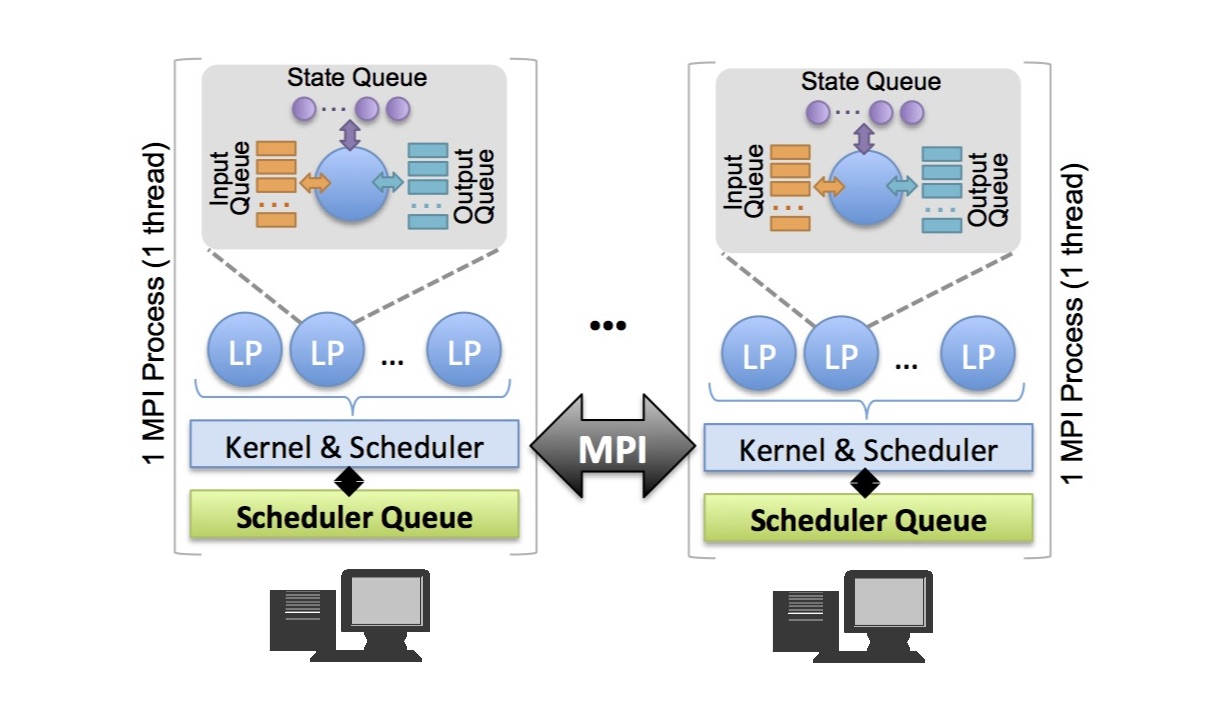
\includegraphics[width=\textwidth]{images/MUSEarch.jpg}
\end{minipage}
\end{figure}

\begin{itemize}
\item Assessment of the data structures will be conducted on MUSE.
\item MUSE performs sequential and optimistically parallel simulations.
\item The kernel handles LP registration, event processing, state saving, synchronization and garbage collection.
\end{itemize}
\end{frame}

\begin{frame}
\frametitle{\centerline{Parallel Simulator Overview}}

A scheduler queue is required to implement four key operations to manage pending events. \\~\\

\begin{itemize}

\item[\ding{182}] \textbf{Enqueue one or more future events}. 

\item[\ding{183}] \textbf{Peek next event}.

\item[\ding{184}] \textbf{Dequeue events for next LP}.

\item[\ding{185}] \textbf{Cancel pending events}.

\end{itemize}   

\end{frame}

\begin{frame}
\frametitle{\centerline{Simulation Model}}

\begin{table}[!ht]\centering \vspace*{-4mm}
\textbf{\caption{Parameters in PHOLD benchmark}}
\begin{tabular}{lp{2.2in}}
\toprule
Parameter & Description \\
\midrule

\textbf{rows} & Total number of rows in model. \\

\textbf{cols} & Total number of columns in model. \#LPs = \textbf{rows} x  \textbf{cols} \\

\textbf{eventsPerLP} & Initial number of events per LP. \\

\textbf{delay} or $\lambda$ & Value used with distribution -- Lambda
($\lambda$) value for exponential distribution \textit{i.e.,}
$P(x|\lambda)=\lambda e^{-\lambda x}$. \\

\textbf{\%selfEvents} & Fraction of events LPs send to self \\

\textbf{granularity} & Additional compute load per event. \\

\textbf{imbalance} & Fractional imbalance in partition to have more LPs on a MPI-process. \\

\textbf{simEndTime} & GVT when simulation logically ends.\\

\bottomrule
\end{tabular}
\end{table}
\end{frame}

\begin{frame}
\frametitle{ \centerline{Scheduler Queues}}
\begin{itemize}
\item MUSE contains 6 scheduling queues for managing pending events.
\item The queues are classified into two categories: single-tier and multi-tier queues.
\item Single-tier queues use only a single data structure to implement the 4 key operations.
\item Multi-tier queues organizes events into tiers and each tier is implemented using different data structures.
\end{itemize}
\end{frame}

\begin{frame}
\frametitle{\centerline{Binary Heap (\textbf{heap})}} 

\begin{figure}
\centering
\begin{minipage}{0.45\textwidth}
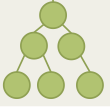
\includegraphics[width=.75\linewidth]{images/binaryHeap.png}
\end{minipage}
\centering
\begin{minipage}{0.45\textwidth}
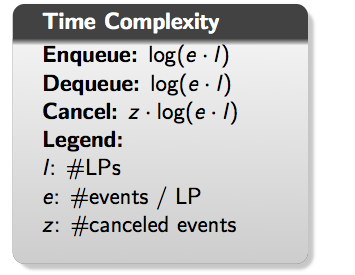
\includegraphics[width=.95\linewidth]{images/complexityHeap.png}
\end{minipage}
\end{figure}

\begin{itemize}
\item It is a single-tier data structure that it is implemented as an array object.
\item A std::vector is used as the backing container and C++11 algorithms (std::push\_heap, st::pop\_heap) are used to maintain the heap.
\item The heap is prioritized based on time stamp with the lowest time stamp at the root of the heap.
\end{itemize}
\end{frame}

\begin{frame}
\frametitle{\centerline{2-tier Heap (\textbf{2tHeap})}}

\begin{figure}
\centering
\begin{minipage}{0.45\textwidth}
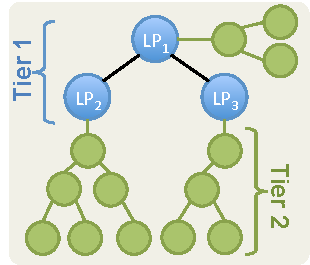
\includegraphics[width=.75\linewidth]{images/2tierQ.pdf}
\end{minipage}
\centering
\begin{minipage}{0.45\textwidth}
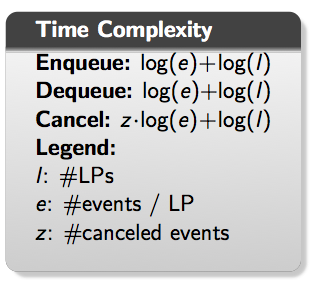
\includegraphics[width=.75\linewidth]{images/complexity2tHeap.png}
\end{minipage}
\end{figure}

\begin{itemize}
\item 2tHeap was designed to reduced the time complexity of cancel operations by subdividing events into two  distinct tiers.
\item The first tier has containers for each local LP on an MPI-process.
\item Each of the the tier-1 containers has a heap of events to be processed by a given LP.
\item A std::vector is used as the backing container for both tiers and standard algorithms are used to maintain the min-heap property for both tiers after each operation.
\end{itemize}
\end{frame}

\begin{frame}
\frametitle{\centerline{2-tier Fibonnaci Heap (\textbf{fibHeap})}}

\begin{figure}
\centering
\begin{minipage}{0.45\textwidth}
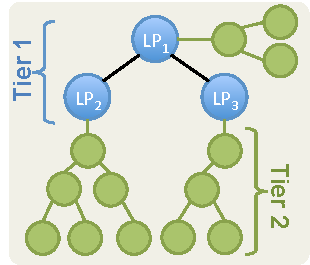
\includegraphics[width=.95\linewidth]{images/2tierQ.pdf}
\end{minipage}
\centering
\begin{minipage}{0.45\textwidth}
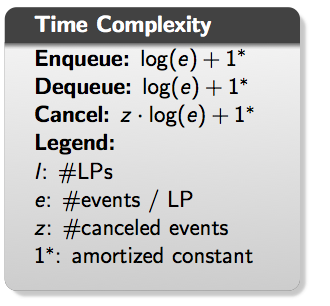
\includegraphics[width=.95\linewidth]{images/complexityfibHeap.png}
\end{minipage}
\end{figure}

\begin{itemize}
\item The fibHeap is an extension of the 2tHeap data structure. It uses a Fibonnaci heap for scheduling LPs.
\item The second tier is a binary heap data structure.
\end{itemize}
\end{frame}

\begin{frame}
\frametitle{\centerline{3-tier Heap (\textbf{3tHeap})}}

\begin{figure}
\centering
\begin{minipage}{0.45\textwidth}
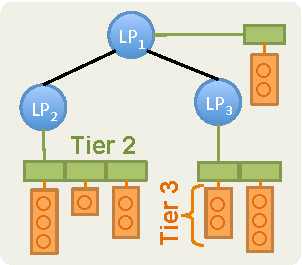
\includegraphics[width=.85\linewidth]{images/3tierQ.pdf}
\end{minipage}
\centering
\begin{minipage}{0.45\textwidth}
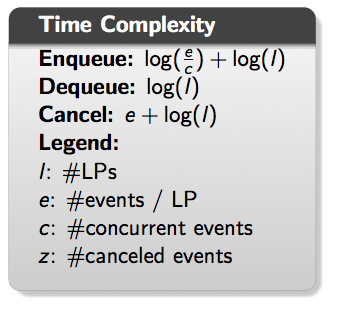
\includegraphics[width=.85\linewidth]{images/complexity3tHeap.png}
\end{minipage}
\end{figure}

\begin{itemize}
\item The 3tHeap builds upon 2tHeap by further subdividing the second tier into two tiers.
\item The binary heap implementation for the first tier that manages LPs for scheduling has been retained from 2tHeap.
\item Assuming each LP has \textit{c} concurrent events on an average, there are $\frac{e}{c}$ tier-2 entries with each one having \textit{c} pending events.
\end{itemize}
\end{frame}

\begin{frame}
\frametitle{\centerline{3-tier Heap (\textbf{3tHeap}) - Enqueue Operation}}
\begin{figure}
\begin{minipage}{0.45\textwidth}
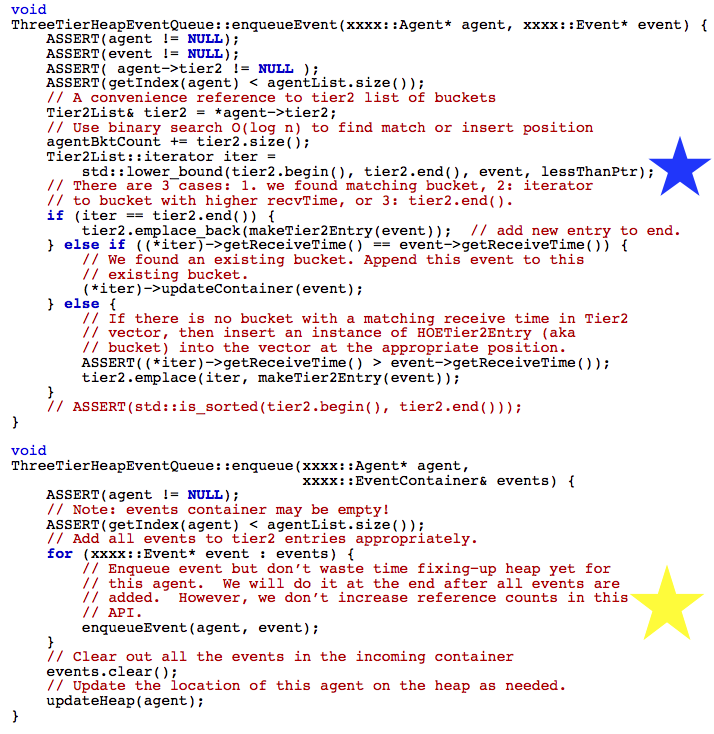
\includegraphics[width=220px, height=220px]{images/3tHeapEnqueueCode.png}
\end{minipage}
\end{figure}
\end{frame}


\begin{frame}
\frametitle{\centerline{Ladder Queue (\textbf{ladderQ})}}

\begin{figure}
\centering
\begin{minipage}{0.45\textwidth}
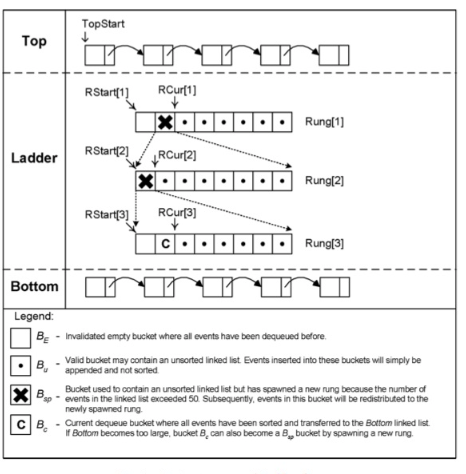
\includegraphics[width=.95\linewidth]{images/LadderQueue.png}
\end{minipage}
\centering
\begin{minipage}{0.45\textwidth}
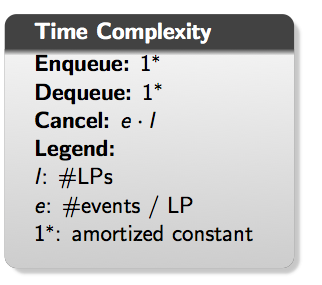
\includegraphics[width=.95\linewidth]{images/complexityLadderQ.png}
\end{minipage}
\end{figure}
\begin{itemize}
\item Ladder Queue is a priority queue implementation proposed by Tang et al. with amortized constant time complexity.
\item There are two key ideas underlying the Ladder Queue, namely: minimize the number of events to be sorted and delay sorting of events as much as possible.
\end{itemize}
\end{frame}

\begin{frame}
\frametitle{\centerline{Ladder Queue (\textbf{ladderQ}) Dequeue Operation}}
\begin{figure}
\centering
\begin{minipage}{0.55\textwidth}
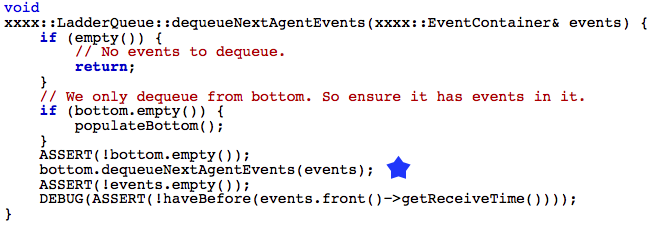
\includegraphics[width=190px, height=105px]{images/dequeueBottomLadderQ.png}
\end{minipage}
\centering
\begin{minipage}{0.45\textwidth}
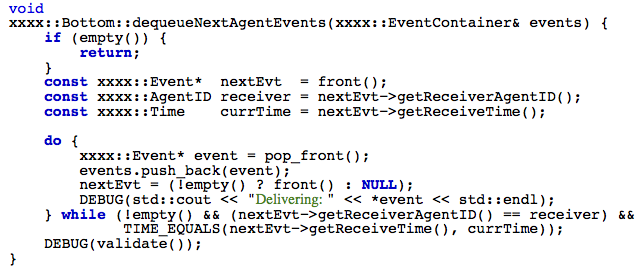
\includegraphics[width=190px, height=105px]{images/botDequeueLadderQcode.png}
\end{minipage}
\end{figure}
\end{frame}

\begin{frame}
\frametitle{\centerline{2-tier Ladder Queue (\textbf{2tLadderQ})}}

\begin{figure}
\centering
\begin{minipage}{0.45\textwidth}
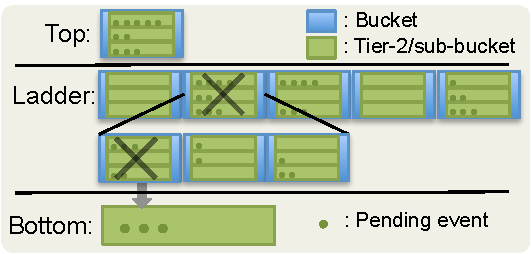
\includegraphics[width=0.99\linewidth]{images/2tLadderQ.pdf}
\end{minipage}
\centering
\begin{minipage}{0.45\textwidth}
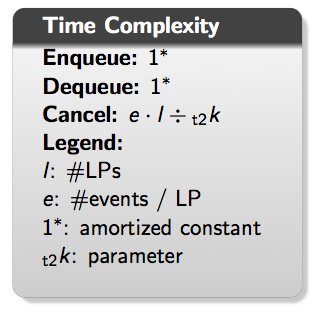
\includegraphics[width=.85\linewidth]{images/complexity2tLadderQ.png}
\end{minipage}
\end{figure}
\begin{itemize}
\item 2-tier Ladder Queue is the proposed alternative to Ladder Queue because the cost of event cancellation during rollbacks is reduced.
\item 2tLadderQ retains the amortized constant time complexity of ladderQ with performance gains during event cancellation.

\end{itemize}
\end{frame}

\begin{frame}
\frametitle{\centerline{2-tier Ladder Queue (\textbf{2tLadderQ}) Cancel Operation}}

\begin{figure}
\centering
\begin{minipage}{0.55\textwidth}
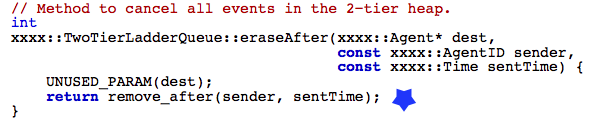
\includegraphics[width=190px, height=35px]{images/eraseAfter2tLadderQcode.png}
\end{minipage}
\centering
\begin{minipage}{0.45\textwidth}
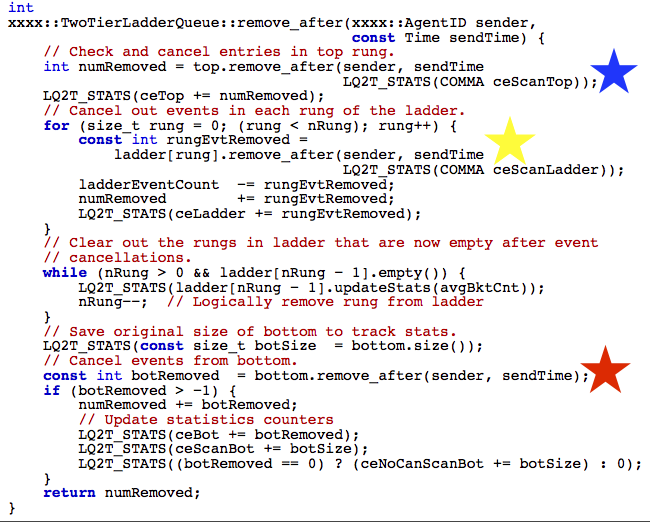
\includegraphics[width=190px, height=155px]{images/removeAfter2tLadderQcode.png}
\end{minipage}
\end{figure}
\end{frame}

\begin{frame}
\frametitle{\centerline{Preliminary Sequential Simulation Results}}
\begin{figure}
\centering
\begin{minipage}{0.75\textwidth}
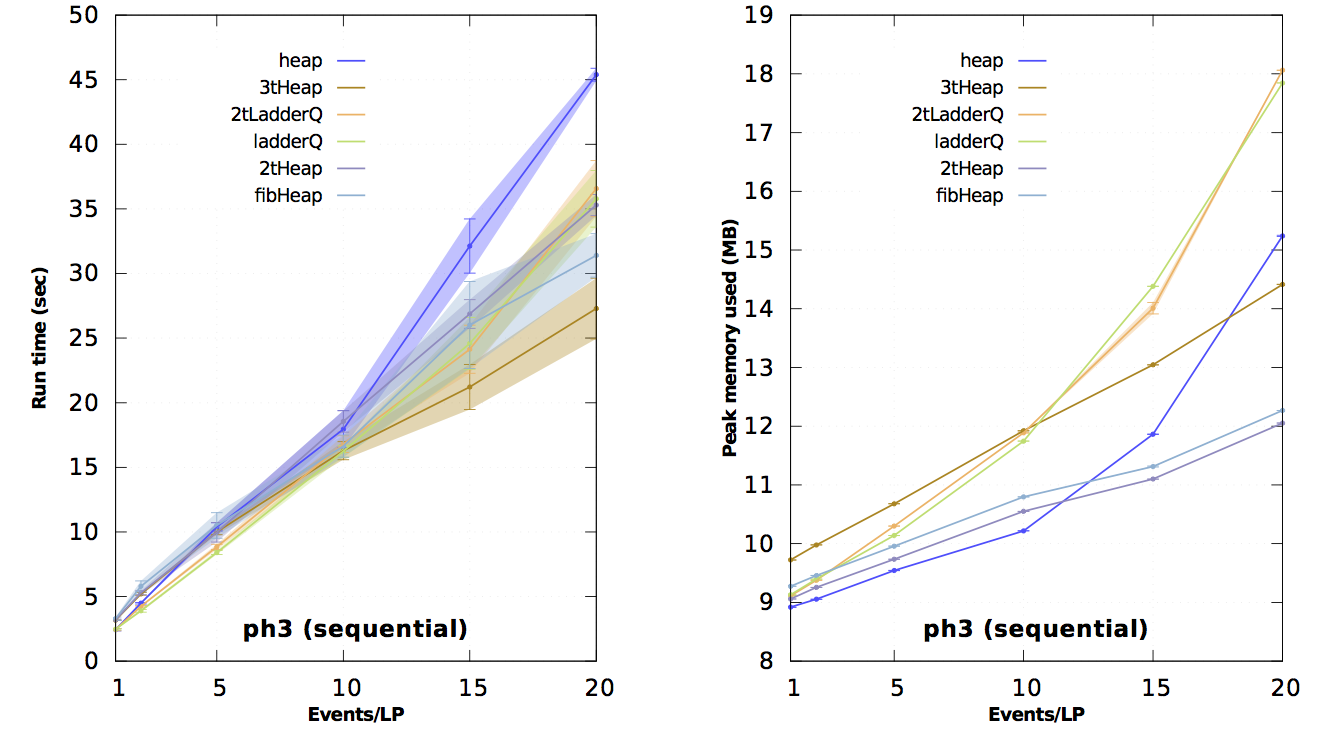
\includegraphics[width=0.85\linewidth]{images/seq.png}
\end{minipage}
\centering
\begin{minipage}{0.35\textwidth}
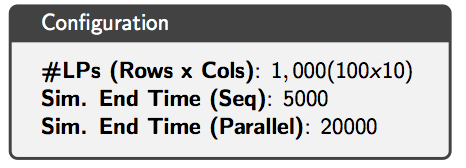
\includegraphics[width=0.85\linewidth]{images/configuration}
\end{minipage}
\end{figure}

\begin{itemize}
\item Sequential simulation run time and peak memory usage statistics is shown with \textbf{\%Self-events} = 25\% and \textbf{$\lambda=1$} at varied values for \textbf{eventsPerLP}.
\end{itemize}
\end{frame}

\begin{frame}
\frametitle{\centerline{Preliminary Parallel Simulation Results}}

\begin{figure}
\centering
\begin{minipage}{0.35\textwidth}
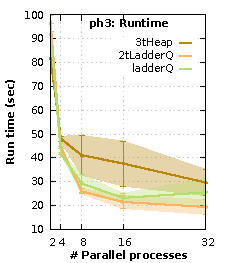
\includegraphics[width=0.85\linewidth]{images/ph3_Delay_10_Evt_10_run_time.pdf}
\end{minipage}
\centering
\begin{minipage}{0.35\textwidth}
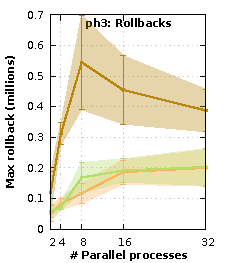
\includegraphics[width=0.85\linewidth]{images/ph3_Delay_10_Evt_10_rollbacks.pdf}
\end{minipage}
\centering
\begin{minipage}{0.35\textwidth}
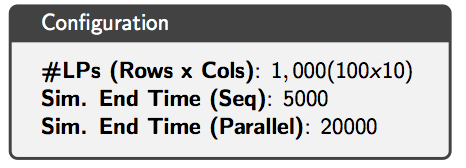
\includegraphics[width=0.85\linewidth]{images/configuration.png}
\end{minipage}
\end{figure}

\begin{itemize}
\item Statistics from parallel simulation with  \textbf{\%Self-events} = 25\%, \textbf{$\lambda=10$} and \textbf{eventsPerLP} = 10. 
\end{itemize}

\end{frame}

\begin{frame}
\frametitle{\centerline{Experiment Design}}
\begin{itemize}
\item Assessments of the effectiveness of the six scheduler queues will be performed by running different configurations of the PHOLD benchmark in sequential and optimistically parallel simulations.
\\~\\
\item Due to a large number of PHOLD parameters and combinations of their values. We will identify the most influential PHOLD parameters that impact performance of the scheduler queues using \textbf{Generalized Sensitivity Analysis}.\\~\\
\item The data to be collected and assessed consists of \textbf{simulation run time} and \textbf{peak memory usage}.
\end{itemize}
\end{frame}

\begin{frame}
\frametitle{\centerline{Plan of Action \& Milestones}}

\begin{itemize}
\item[\ding{182}] \textbf{Sequential \& parallel simulation assessment}: Data will be collected to assess the effectiveness of the different data structures in sequential and parallel simulations. Data collection and analysis for sequential simulations will be completed by 14 March 2017. Data collection and analysis for parallel simulations will be completed by 22 March 2017. \\~\\

\item[\ding{183}] \textbf{ Implement 2 additional simulation models}: We will extend the experimental analysis to include 2 additional models in order to evaluate performance of the data structures across different simulation models. The 2 simulation models will be implemented by 30 March 2017.
\end{itemize}
\end{frame}

\begin{frame}
\frametitle{\centerline{Plan of Action \& Milestones}}

\begin{itemize}

\item[\ding{184}] \textbf{Assessment using additional simulation models}: The assessment of data structure performance using the models in sequential and optimistic parallel simulations will be completed by 28 April 2017.\\~\\

\item[\ding{185}] \textbf{Record experimental results and analysis}: The research thesis writing will be completed by 19 May 2017 in preparation for the thesis defense.

\end{itemize}
\end{frame}

\begin{frame}
\frametitle{References}
\footnotesize{
\begin{thebibliography}{99}\vspace*{-3.5mm}
\bibitem[Dickman et al., 2013]{p1} Dickman et al., (2013) Event Pool Structures for PDES on Many-core Beowulf Clusters. \emph{In Proceedings of the 1st ACM SIGSIM Conference on Principles of Advanced Discrete Simulation} ACM, New York, NY, USA, 103-114.

\bibitem[Franceschini et al., 2015]{p1} Franceschini et al., (2015) A Comparative Study of Pending Event Set Implementations for PDEVS Simulation. \emph{In Proceedings of the Symposium on Theory of Modeling and Simulation} Society for Computer Simulation International San Diego, CA, USA, 77-84.

\bibitem[Gupta et al., 2014]{p1} Wilsey et al., (2014) Lock-free Pending Event Set Management in Time Warp. \emph{In Proceedings of the 2nd ACM SIGSIM Conference on Principles of Advanced Discrete Simulation} ACM, New York, NY, USA, 15-26.

\bibitem[Jafer et al., 2013]{p1} Jafer et al., (2013) Synchronization methods in parallel and distributed discrete-event simulation{ Simulation Modeling Practice and Theory} 30(2013), 54-73.

\bibitem[Marotta et al., 2016]{p1} Marotta et al., (2016) A Non-Blocking Priority Queue for the Pending Event Set.{In Proceedings of the 9th EAI International Conference on Simulation Tools and Techniques} ICST, Brussels, Belgium, 46-55.

\bibitem[Tang et al., 2005]{p1} Tang et al., (2005) Ladder Queue: An O(1) Priority Queue Structure for Large-scale Discrete Event Simulation.{ACM Trans. Model. Comput. Simul.} 15, 3(July 2005), 175-204.
\end{thebibliography}
}
\end{frame}

%------------------------------------------------

\begin{frame}
\Huge{\centerline{The End}}
\end{frame}

%----------------------------------------------------------------------------------------
\begin{frame}
\frametitle{\centerline{Intro to Discrete Event Simulation (DES)}}
\textbf{Discrete Event Simulation (DES)} is a framework for simulating the behavior of real or imagined systems.
\begin{block}{Simulation properties}
\begin{itemize}
\item an \textbf{entity} that is an object of interest in the simulated system.
\item a \textbf{state} that is represented by a set of variables that describe the system at a particular point in time.
\item an \textbf{event} that is an instantaneous occurrence that can change the state of the simulated system. 
\item a virtual simulation \textbf{clock} that indicates the time of the last event occurrence that has been simulated. 
\item an \textbf{evolution} of the modeled system that is given by a chronologically ordered sequence of events.\newline
\textbf{\textit{s}\textsubscript{0}, (\textit{e}\textsubscript{0}, \textit{t}\textsubscript{0}), \textit{s}\textsubscript{1},
(\textit{e}\textsubscript{1}, \textit{t}\textsubscript{1}),
\textit{s}\textsubscript{2},(\textit{e}\textsubscript{2},
\textit{t}\textsubscript{2}), ......., \textit{s}\textsubscript{n},(\textit{e}\textsubscript{n},
\textit{t}\textsubscript{n})}
\end{itemize}
\end{block}
\end{frame}

\begin{frame}
\frametitle{\centerline{Intro to Discrete Event Simulation (DES)}}
\begin{block}{Simulation application}
\begin{itemize}
\item The model of the real or imagined system.
\item The collection of state variables.
\item The collection of event handlers.
\end{itemize}
\end{block}

\begin{block}{Simulator}
\begin{itemize}
\item The environment that manages and executes the simulation.
\item Maintains an event list for handling events.
\item Manages forward progress of simulation time.
\end{itemize}
\end{block}

\end{frame}

\begin{frame}
\frametitle{\centerline{Implementation of DES}}

\begin{figure}[T]\vspace*{-0.5cm}
\begin{minipage}[b]{0.85\textwidth}
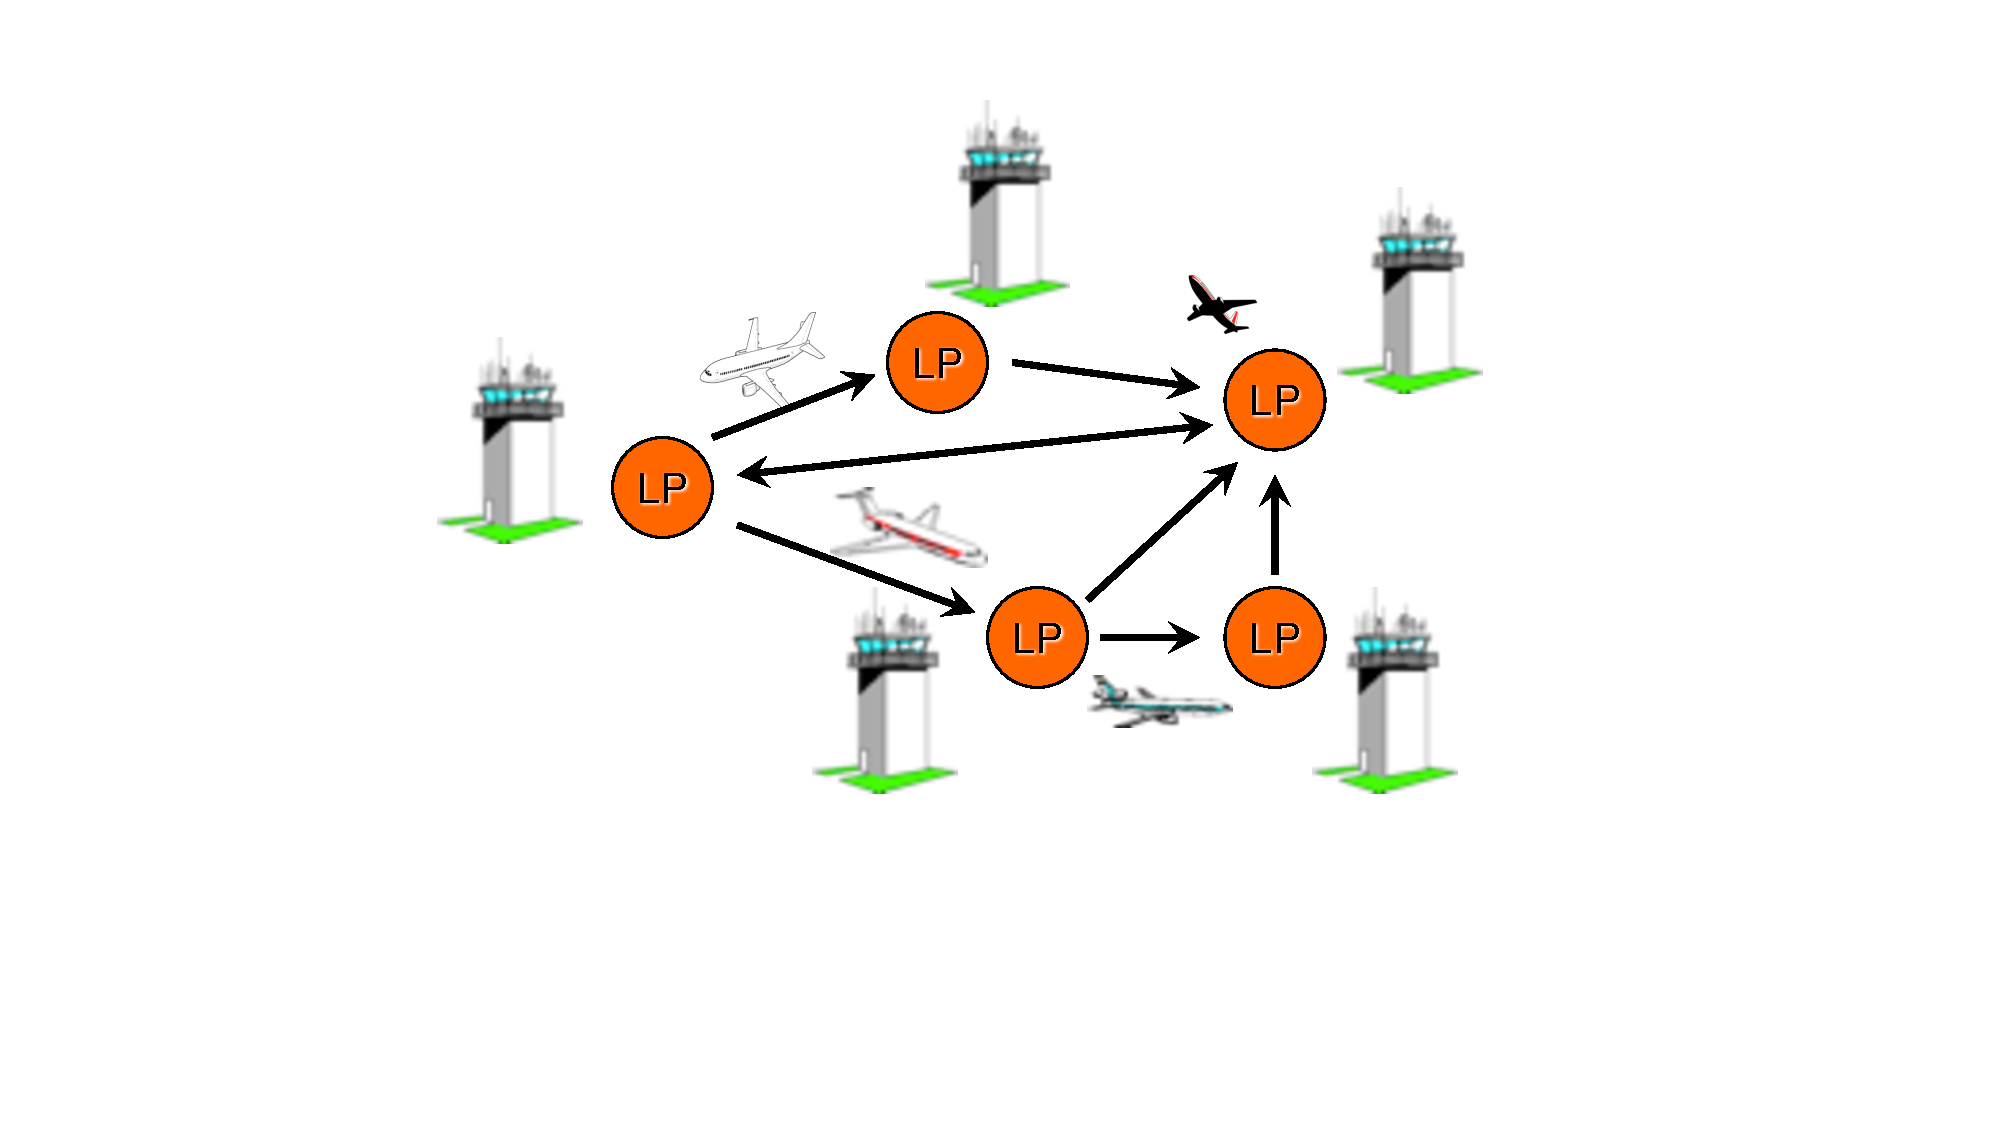
\includegraphics[width=\textwidth]{images/Airport.pdf}
\end{minipage}
\end{figure}
\begin{itemize}\vspace*{-2cm}
\item  DES is implemented as a set of logical processes (LPs).
\item LPs map to physical processes in the simulated system.
\item Each LP has the following components:\\
\hspace*{7mm}\textbf{state queue}: maintains saved states of the LP.\\
\hspace*{7mm}\textbf{input queue}: maintains events received from other LPs.\\
\hspace*{7mm}\textbf{output queue}: maintains events sent to other LPs. \\
\hspace*{7mm}\textbf{local clock}: time of last event processed.

\end{itemize}
\end{frame}

\begin{frame}
\begin{figure}[T]\vspace*{-0.5cm}
\begin{minipage}[b]{0.85\textwidth}
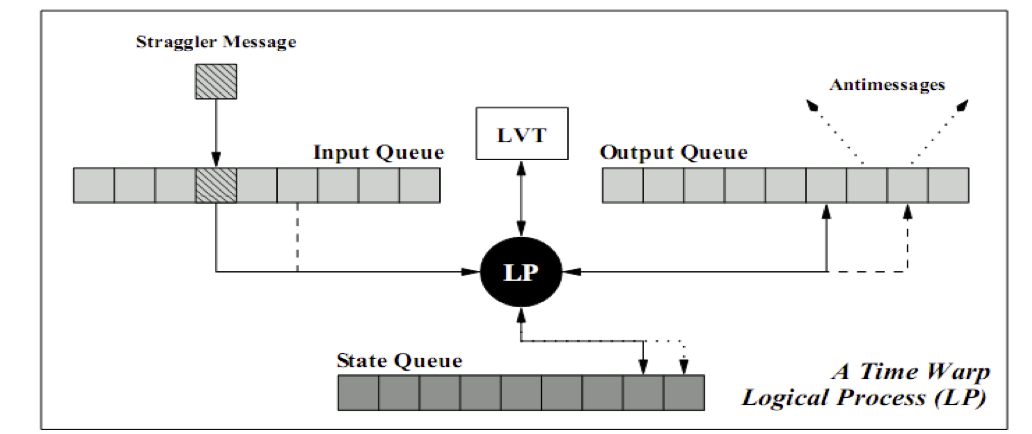
\includegraphics[width=\textwidth]{images/logicalProcess.png}
\end{minipage}
\end{figure}
\end{frame}


\begin{frame}
\frametitle{\centerline{Implementation of DES}}

\begin{figure}[T]\vspace*{-1cm}
\begin{minipage}[b]{0.85\textwidth}
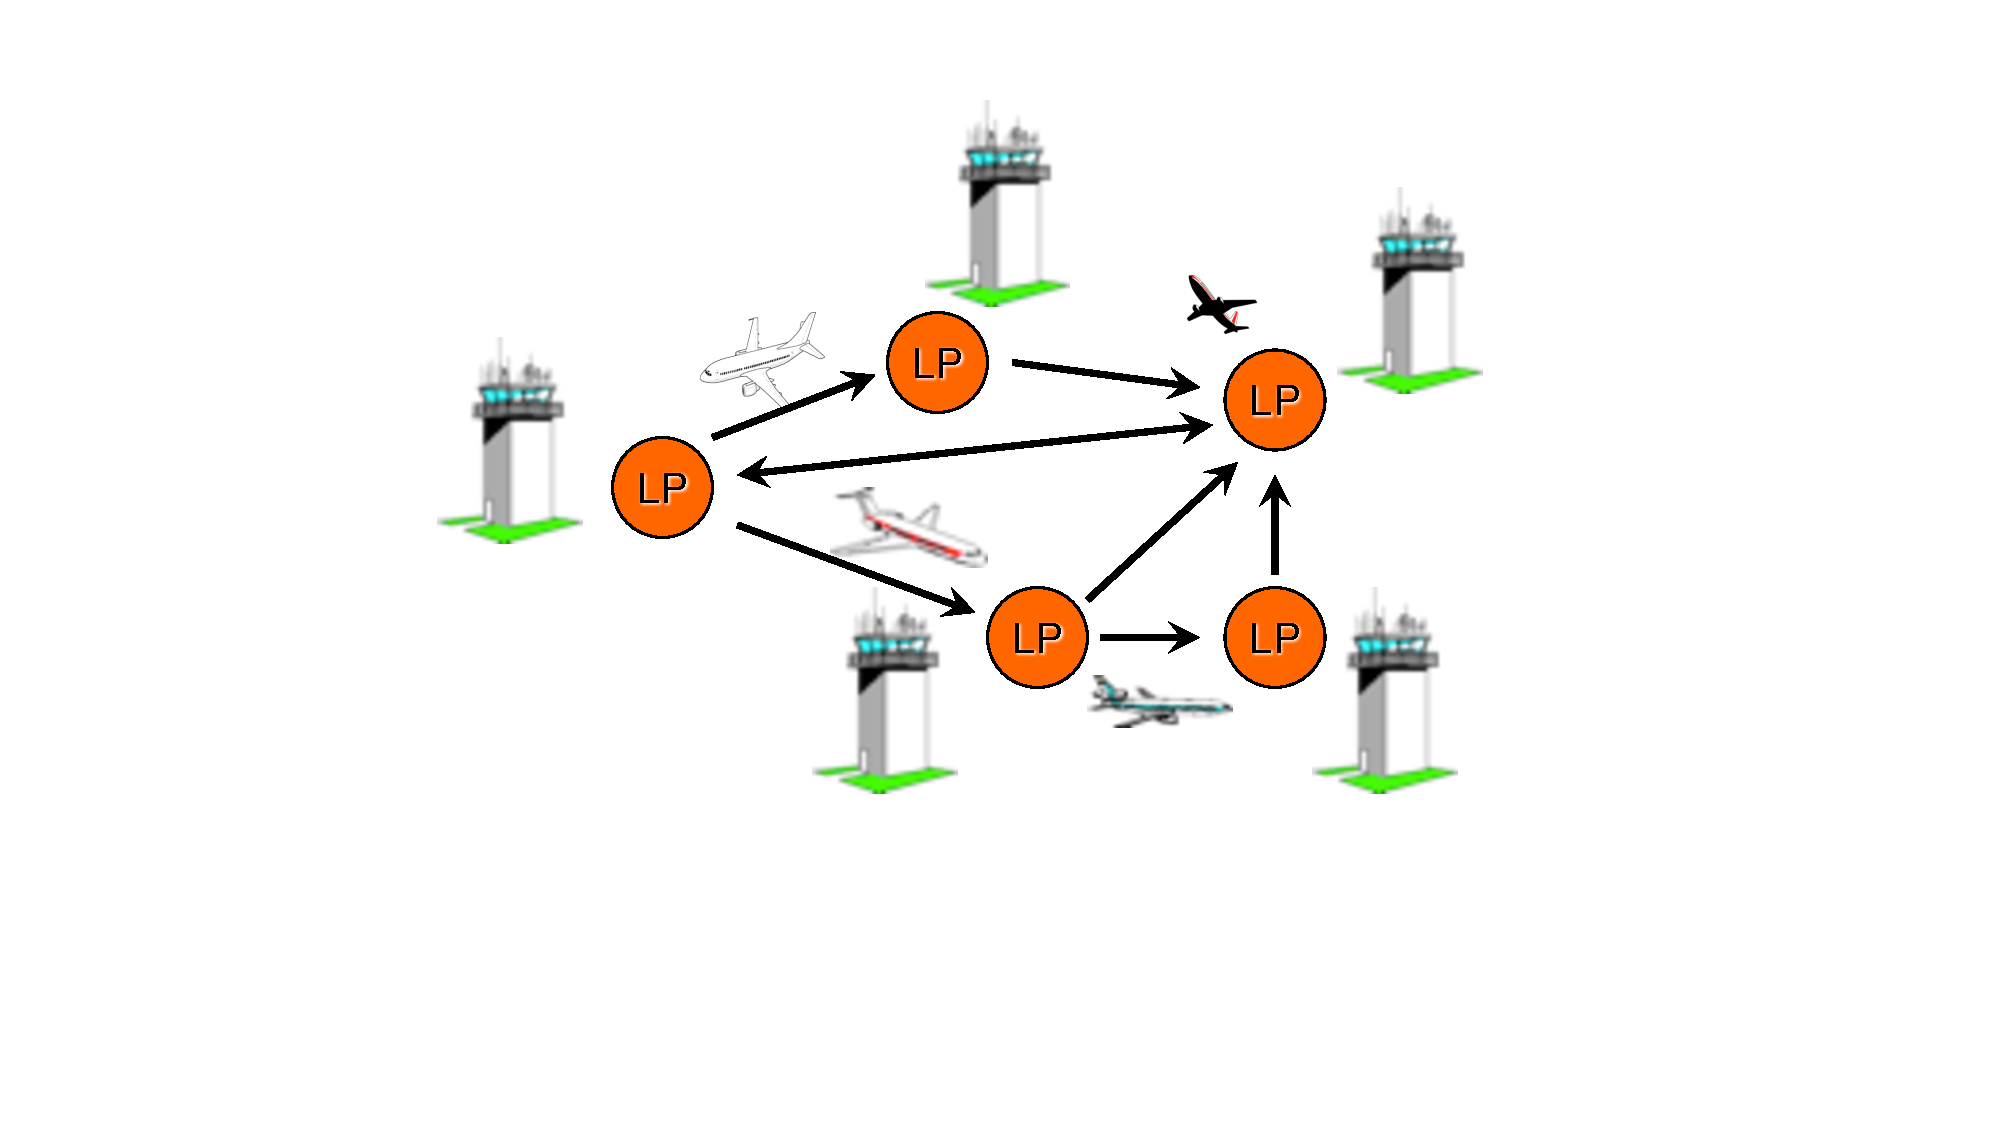
\includegraphics[width=\textwidth]{images/Airport.pdf}
\end{minipage}
\end{figure}
\begin{itemize}\vspace*{-2cm}
\item LPs interact with each other by exchanging and processing time stamped events.
\item Events that are yet to be processed are called \textbf{pending events}. 
\item LPs process these events in time stamp order order and generate new events that are transmitted to other LPs.
\end{itemize}
\end{frame}

\begin{frame}
\frametitle{\centerline{Parallelism in DES}}

\begin{figure}[T] \vspace*{-0.3cm}
\begin{minipage}[b]{0.85\textwidth}
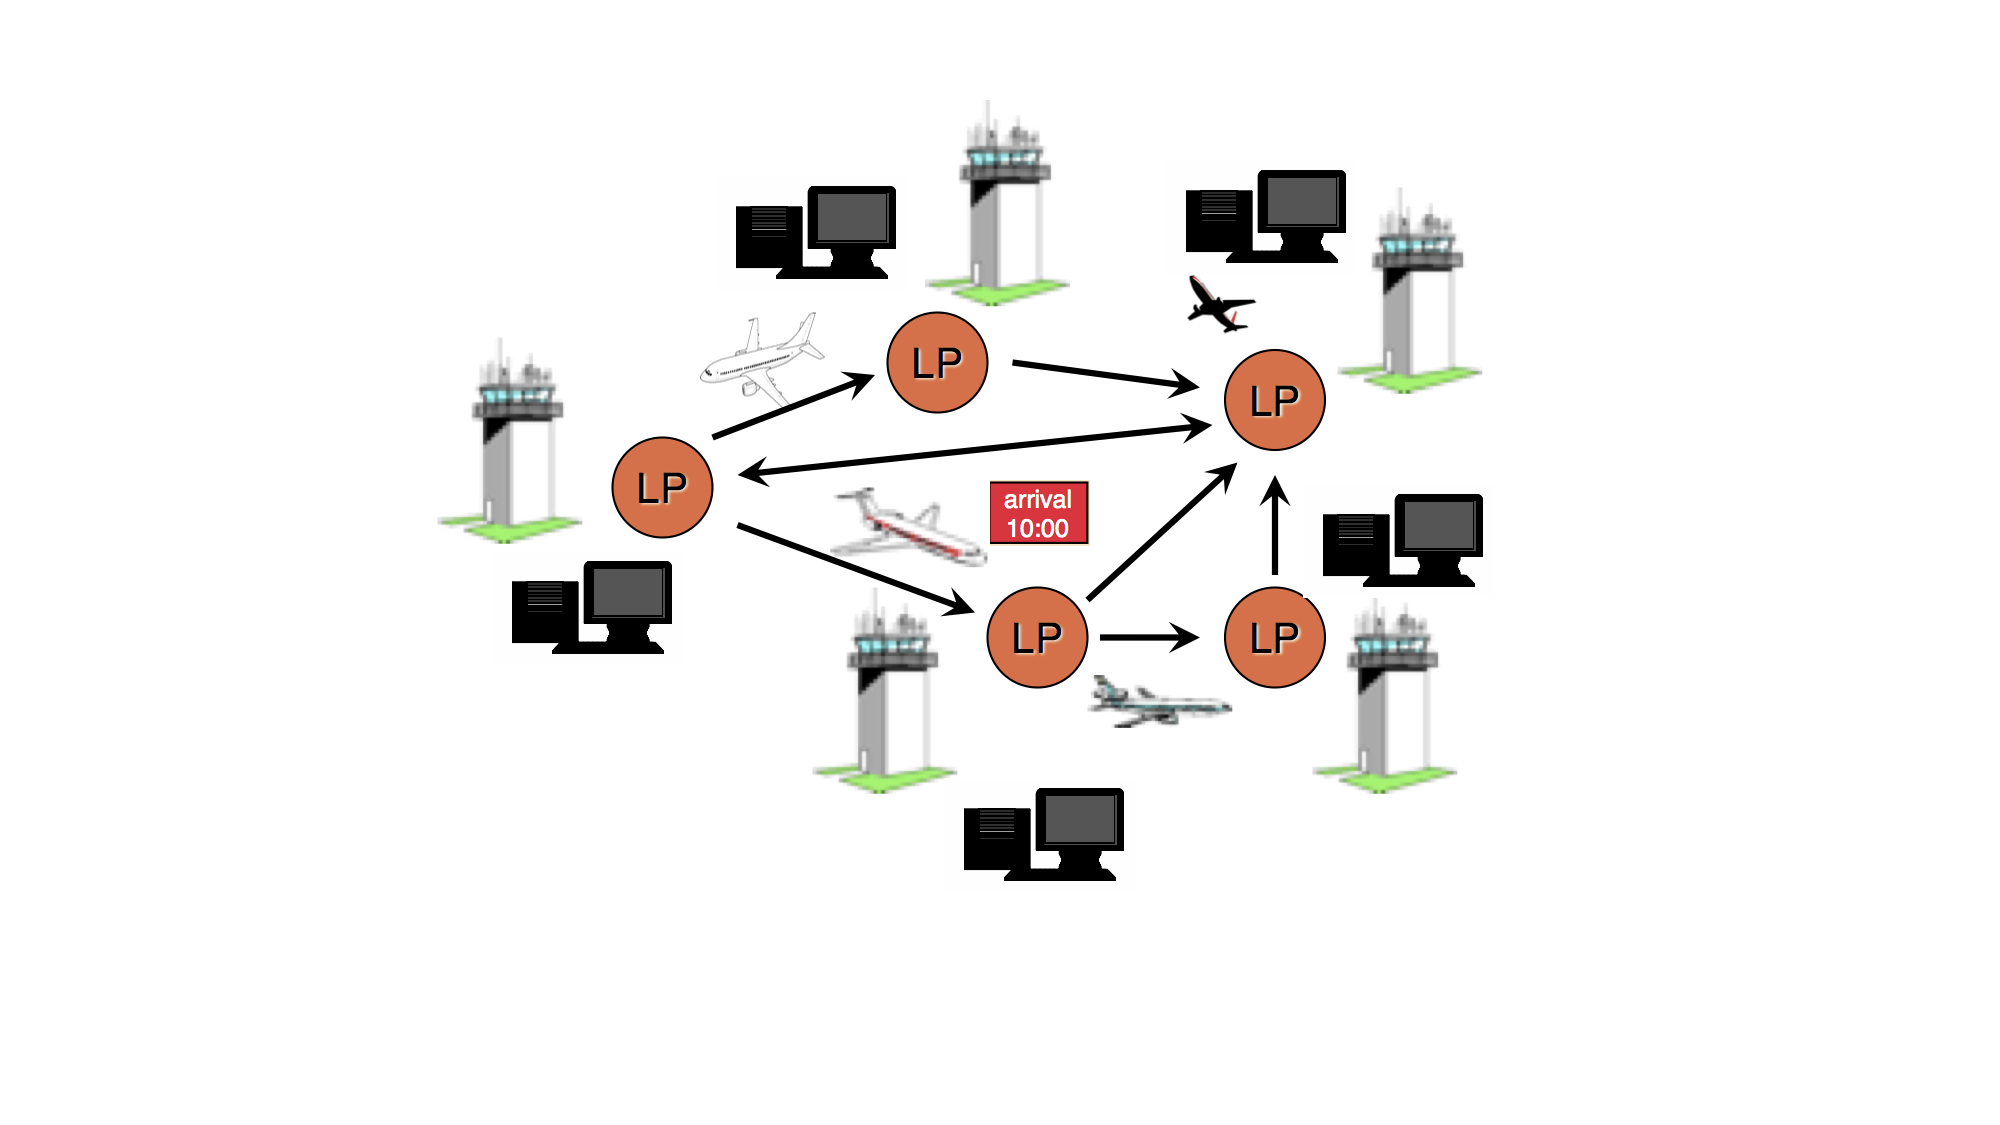
\includegraphics[width=\textwidth]{images/AirportMod.png}
\end{minipage}
\end{figure}

\begin{itemize}\vspace*{-1.5cm}
\item Parallel computing simulates DES models on parallel computers. 
\item In parallel DES (PDES), LPs exchange time stamped events using message passing.
\item Processing events concurrently on different processors is hard.
\item \textbf{Synchronization problem}: since the simulation runs in parallel, all LPs have their own internal clock, so each LP may be at different points in time relative to each other.


\end{itemize}
\end{frame}

\begin{frame}
\frametitle{\centerline{Parallelism in DES}}
\begin{block}{Conservative approach to PDES}
\begin{itemize}
\item Causality errors are not allowed to occur.
\item Strategy required to determine when it is safe to process an event.
\end{itemize}
\end{block}
\begin{block}{Optimistic approach to PDES}
\begin{itemize}
\item Allows causality errors to occur.
\item When a causality error is detected, rollback mechanism is invoked.  
\end{itemize}
\end{block}
\end{frame}

\begin{frame}
\frametitle{\centerline{Ladder Queue (\textbf{ladderQ})}}

\begin{figure}
\centering
\begin{minipage}{0.45\textwidth}
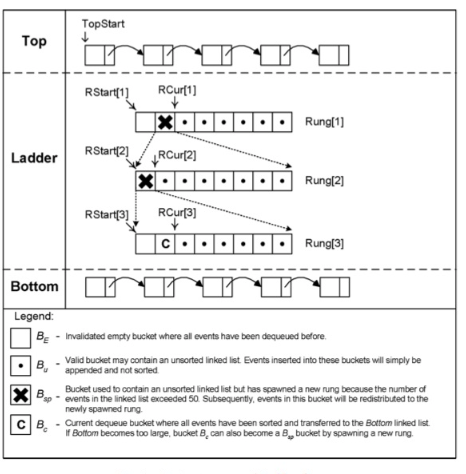
\includegraphics[width=1\linewidth]{images/LadderQueue.png}
\end{minipage}
\centering
\begin{minipage}{0.45\textwidth}
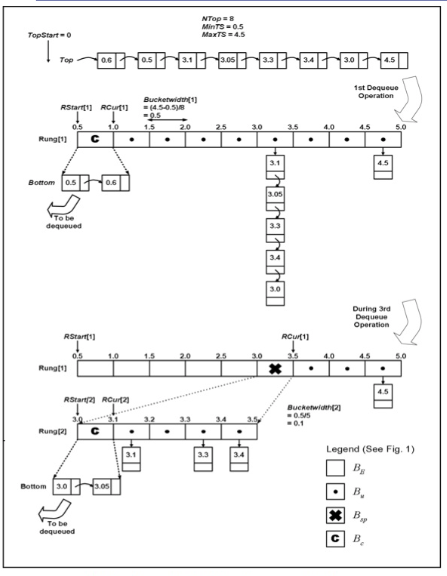
\includegraphics[width=1\linewidth]{images/LadderQueue1.png}
\end{minipage}
\end{figure} 
\end{frame}

\end{document}